\chapter{Magnetism}

\textit{What magnetism is, no-one knows. We can only think of it as a peculiar condition created in space by the motion of electricity.}\\
\noindent\textbf{-   Sydney Evershed}

\vspace{1cm}


\begin{marginfigure}%
  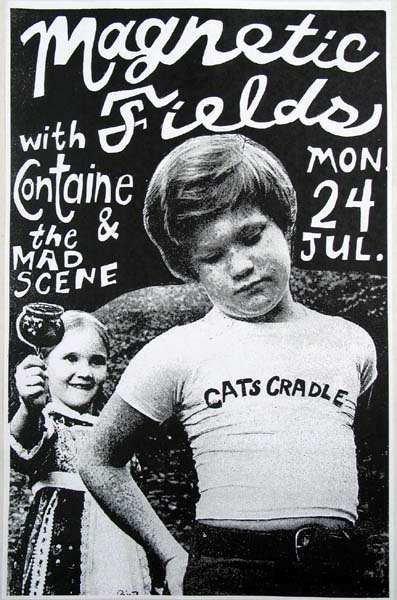
\includegraphics[width=\linewidth]{mag_fields.jpg}
  \caption{Magnetic Fields concert poster}
  \label{fig:marginfig}
\end{marginfigure}

Magnetism is the phenomenon of current interactions.  A current moving through space applies a force to other currents around it.  The story of magnetism is one of the deeper mysteries in physics.  As in electrostatics, physics uses the construct of the vector field to narrate the force interaction.

Currents generate magnetic fields in the space around them.  Currents also interact with fields in space.  This results in a magnetic force.  The story is therefore split into two parts.  How do currents generate fields in space?  How do currents interact with fields in space?  The present narrative addresses the second question first.


\section{Magnetic Force/Field}
Consider a a magnetic field in space $\overrightarrow{B}(\overrightarrow{r})$ and a particle with charge $q$ and velocity $\overrightarrow{v}$.   The resulting magnetic force is represented using the vector cross product.

$$\overrightarrow{F}_{B}=q\overrightarrow{v}\times \overrightarrow{B}$$
Remember the magnitude of the cross product is proportional to the $\sin$ of the angle between the field vector and the velocity vector.
$$F_{B}=qvB \sin \theta$$

\begin{marginfigure}[10pt]
 
\tdplotsetmaincoords{60}{110}
\begin{tikzpicture}[scale=1,tdplot_main_coords]
\coordinate (O) at (0,0,0);
\coordinate (P) at (1,2,3);

\draw[very thick,->] (0,0,0) -- (-2,2,0) node[anchor=south ]{$B$};
\draw[very thick,->] (0,0,0) -- (0,4,0) node[anchor=north west]{$v$};
\draw[very thick,->] (0,0,0) -- (0,0,3) node[anchor=south]{$F_{B}$};
\fill (0,0,0) circle(1mm) node[anchor=north east]{$q$};
%draw a vector from origin to point (P) 
\draw (-0.6,1.2,0) node[anchor=center,color=black]{$\theta$};


%draw projection on xy plane, and a connecting line
%syntax: \tdplotdrawarc[coordinate frame, draw options]{center point}{r}{angle}{label options}{label}
%\tdplotdrawarc{(O)}{0.2}{0}{\phivec}{anchor=north}{$\phi$}


%set the rotated coordinate system so the x'-y' plane lies within the
%"theta plane" of the main coordinate system
%syntax: \tdplotsetthetaplanecoords{\phi}
%\tdplotsetthetaplanecoords{\phivec}

%draw theta arc and label, using rotated coordinate system
%\tdplotdrawarc[tdplot_rotated_coords]{(0,0,0)}{0.5}{0}{\thetavec}{anchor=south west}{$\theta$}

\end{tikzpicture}

  \caption{Force of a moving charged particle in a magnetic field}
  \label{fig:marginfig}
\end{marginfigure}


\subsection{Unit}
The SI unit of magnetic field is the Tesla, named after Serbian-American mad scientist Nikola Tesla.
$$1 \ \text{Tesla}=\frac{1\ \text{Newton}}{1\ \text{Ampere} \cdot \text{meter}}$$

\newpage
\begin{marginfigure}%
  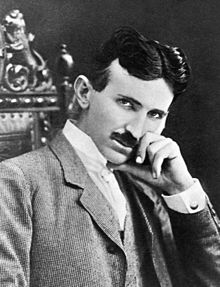
\includegraphics[width=\linewidth]{tesla.jpg}
  \caption{Handsome: Nikola Tesla}
  \label{fig:marginfig}
\end{marginfigure}


\subsection{No Work}
Since the magnetic force is always perpendicular to the velocity (displacement) no work is done by a static magnetic field on a moving particle.
$$W_B=\sum \overrightarrow{F}_B\cdot \ \Delta\overrightarrow{s}=\sum \overrightarrow{F}_B\cdot\overrightarrow{v}\ \Delta t=0$$
Fields may do work on magnetic dipoles, namely loops of current, but these are rigid bodies.  A constant magnetic field does not work on a single moving charged particle.
\section{Magnetic Force on a Straight Wire }
For $N$ charges particle in wire of length $L$ and cross-sectional area $A$, the total force on the wire is given as follows.

$$\overrightarrow{F}_{wire}=Nq\overrightarrow{v}\times \overrightarrow{B}= (nAL)q\overrightarrow{v}\times \overrightarrow{B}$$ 
Recall the expression for current as a charge rate of flux.  
$$I=nqvA=\overrightarrow J \cdot \overrightarrow A $$
In this way the force can be expressed in terms of the current and the length of the wire.  Since the force is a vector product each factor in the product must be a vector.  since the current is technically a scalar we vectorize the length in the notation.  Of course a length by itself is not a true vector but rather a pseudo-vector.  The sign which lifts the ambiguity for the direction of the $\overrightarrow{L}$ vector is borrowed from the sign of the scalar current $I$.
$$\overrightarrow{F}_{wire}=I\overrightarrow{L}\times\overrightarrow{B} $$


\begin{marginfigure}%
  
 \tikzset{->-/.style={decoration={
  markings,
  mark=at position #1 with {\arrow{latex}}},postaction={decorate}}}
  
\begin{tikzpicture}[scale=1]
\draw[very thick,->-=.5] (0,3) -- (0,0) node[midway, anchor=west]{$I$};

\draw[->] (-1,0.3)--(-0.2,0.3);
\draw[->] (-1,0.5)--(-0.2,0.5);
\draw[->] (-1,0.7)--(-0.2,0.7);
\draw[->] (-1,0.9)--(-0.2,0.9);
\draw (-1,0.6) node[anchor=east]{$B$};

\begin{scope}[scale={1}, shift={(0.4,0.6)}]
\draw (0,0) circle(1.8mm);
\fill (0,0) circle(0.3mm);
\draw (0.2,0) node[anchor=west]{$F$};
\end{scope}
\end{tikzpicture}


  \caption{Magnetic force on a current carrying wire }
  \label{fig:marginfig}
\end{marginfigure}



\section{General Wire}
For a general wire of any shape the approach is to break it up into small pieces of current carrying wire $\Delta\overrightarrow{s}$ and calculate the force $\Delta\overrightarrow{F}_{wire}$ on each piece.  We use the variable $i$ as an index for the pieces. 
$$\Delta\overrightarrow{F}_{i}=I\ \Delta\overrightarrow{s}_i\times\overrightarrow{B}(\overrightarrow{r}_i) $$
To calculate the total force a sum over the index $i$ is taken.  This add up all the little vector forces into a total force vector $\overrightarrow{F}_{wire}$.
$$\overrightarrow{F}_{wire}=\sum_i \Delta\overrightarrow{F}_{i}=\sum_i I\ \Delta\overrightarrow{s}_i\times\overrightarrow{B} (\overrightarrow{r}_i)$$
\newpage

\marginnote{One of the first drawings of a magnetic field, by Ren� Descartes, 1644. It illustrated his theory that magnetism was caused by the circulation of tiny helical particles, "threaded parts", through threaded pores in magnets.}

\begin{marginfigure}[20pt]%
  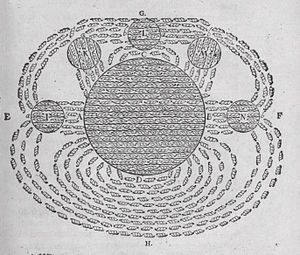
\includegraphics[width=\linewidth]{descartes_field.jpg}
  \caption{Descartes 1644 representation of the magnetic field}
  \label{fig:marginfig}
\end{marginfigure}

\subsection{Uniform Static Field: Path Independence}
A uniform and static magnetic field is constant over space and time.  $\overrightarrow{B} (\overrightarrow{r}_i)=\overrightarrow{B} $ so the summation is only on the path elements and dependent on spatial variation in the magnetic field. Such a field generates no net force.
$$\overrightarrow{F}_{wire}=I \left(\sum_a^b \ \Delta\overrightarrow{s} \right) \times\overrightarrow{B} =I\overrightarrow{s}_{ab}\times\overrightarrow{B} $$
 Such a field generates no net force.  This is because a loop has the same beginning point and end point.
$$\overrightarrow{F}_{wire}=I \left(\sum_a^a \ \Delta\overrightarrow{s} \right) \times\overrightarrow{B}=0 $$


\section{Torque on a Current Loop}
 
 \begin{marginfigure}[20pt]%

 
 \tikzset{->-/.style={decoration={
  markings,
  mark=at position #1 with {\arrow{latex}}},postaction={decorate}}}
  
\begin{tikzpicture}[scale=1]
\draw[very thick,->-=.5] (0,0) -- (2,0);
\draw[very thick,->-=.5] (2,0) -- (2,3)node[midway, anchor=west]{$I$};
\draw[very thick,->-=.5] (2,3) -- (0,3) ;
\draw[very thick,->-=.5] (0,3) -- (0,0);
\draw[->] (-1,0.3)--(-0.2,0.3);
\draw[->] (-1,0.5)--(-0.2,0.5);
\draw[->] (-1,0.7)--(-0.2,0.7);
\draw[->] (-1,0.9)--(-0.2,0.9);
\draw (-1,0.6) node[anchor=east]{$B$};

\begin{scope}[scale={1}, shift={(-0.4,2.4)}]
\draw (0,0) circle(1.8mm);
\fill (0,0) circle(0.3mm);
\draw (-0.2,0) node[anchor=east]{$F_1$};
\end{scope}

\begin{scope}[scale={1}, shift={(2.4,2.4)}]
\draw (0,0) circle(1.8mm);
\fill (0,0) circle(0.3mm);
\draw (0.2,0) node[anchor=west]{$F_2$};
\begin{scope}[scale={1}, rotate={(45)}]
\draw(-0.18,0) -- (0.18,0);
\draw(0,-0.18) -- (0,0.18);
\end{scope}
\end{scope}
\end{tikzpicture}

  \caption{Torque on a closed loop}
  \label{fig:marginfig}
\end{marginfigure}
While the total force is zero for a uniform magnetic field on a closed current loop there is a net torque on the loop.  Consider a rectangular loop of current with area $A$ and uniform magnetic field $B$.  The total torque is the product of the area and the magnetic field. 
$$ \tau=IAB$$
$$ \overrightarrow{\tau}=I\overrightarrow{A}\times \overrightarrow{B}$$
\subsection{Magnetic Moment}
The magnetic moment is defined as product of the current and the area.  Note that the current is a scalar and area is a vector.  Thus the magnetic moment is a vector quantity.
$$\overrightarrow{\mu}= I \overrightarrow{A}$$
The torque on the loop may be parameterized in terms of the magnetic moment.
$$\overrightarrow{\tau}=\overrightarrow{\mu}\times \overrightarrow{B}$$
\section{Homopolar Electric Motor}
The homopolar motor was the first electrical motor to be built. Its operation was demonstrated by Michael Faraday in 1821 at the Royal Institution in London.  It is driven by a Lorentz force.  A paper clip, AAA battery and permanent magnet constitute a homopolar motor.
\begin{marginfigure}[-180pt]%
  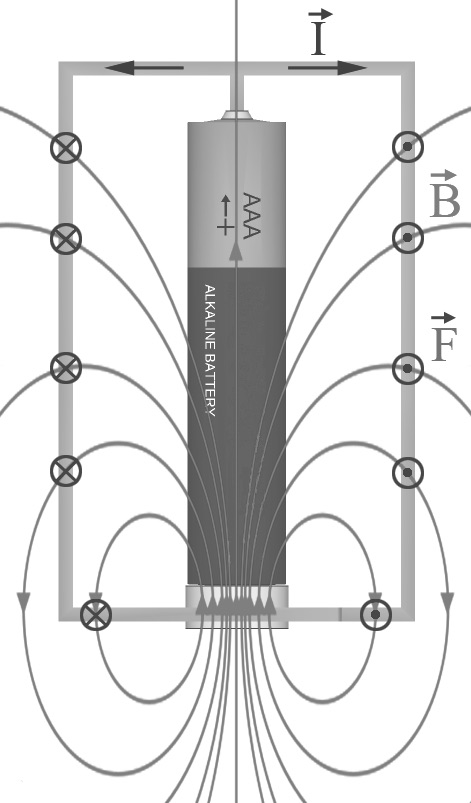
\includegraphics[width=\linewidth]{homopolar_motor.jpg}
  \caption{Simple homopolar motor}
  \label{fig:marginfig}
\end{marginfigure}


\newpage
\section{Circular Motion of a Charged Particle in a Uniform B Field}
\begin{marginfigure}[0pt]%
  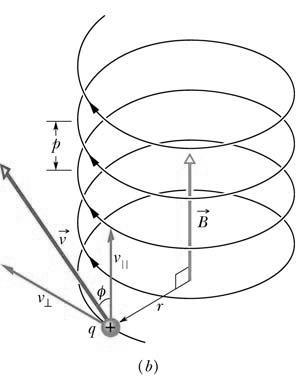
\includegraphics[width=\linewidth]{helix.jpg}
  \caption{Helical motion of a charged particle in a magnetic field}
  \label{fig:marginfig}
\end{marginfigure}
$$F_B=F_c$$
$$ qv_{\perp}B=\frac{mv_{\perp}^2}{r}$$
$$\frac{v_{\perp}}{r}=\omega=\frac{qB}{m}$$
\section{General Motion}
The total force on an electric field and magnetic field on a moving charged particle is known as the Lorentz force.
$$\overrightarrow{F}=q\overrightarrow{E}+q\overrightarrow{v}\times\overrightarrow{B}$$
\section{Velocity Selector}
For perpendicular electric and magnetic fields the Lorentz force will be zero on particle on a particle traveling with a perpendicular component of velocity equal to the ratio of electric field to magnetic field.
$$\overrightarrow{E}=E\hat{x} \hspace{1cm} \overrightarrow{B}=B\hat{y} \hspace{1cm} \overrightarrow{v}=v\hat{z}$$
$$\overrightarrow{F}=qE\hat{x}+qvB\hat{z}\times\hat{y}=q(E-vB)\hat{x}$$
$$v=\frac{E}{B}$$

\begin{marginfigure}
  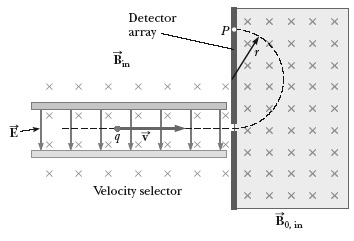
\includegraphics[width=\linewidth]{selector.jpg}
  \caption{Mass spectroscopy with a velocity selector and a detector plate in a constant magnetic field }
  \label{fig:marginfig}
\end{marginfigure}


\section{Mass Spectroscopy}
Mass spectroscopy leverages the physics of the velocity selector and circular motion in a magnetic field to precisely measure mass to charge ratio.  The radius of curvature of the particle is $r$.
$$r=\frac{mv}{qB}$$
Therefore measuring the electric field, magnetic field and radius of curvature would determine the mass to charge ratio of the particle.

$$\frac{m}{q}=\frac{rB}{v}=\frac{rB^2}{E}$$ 
\section{Sources of Magnetic Field}
Up until now there have only been description of currents interacting with existing magnetic fields.  The second half of the story of magnetism addresses how those fields are generated.

The general law for determining the magnetic field in space $\overrightarrow{B}(\overrightarrow{r})$ generated by a current through a general wire is complex and cumbersome.  We begin with a description of the little bit of magnetic field $ \Delta \overrightarrow{B}$ generated by a current $I$ traveling through a small length of wire $\overrightarrow{s}$.  The vector from the the section of wire to the point in space is $\overrightarrow{r}$.  This is known as the Biot-Savart law.
$$\text{Biot-Savart Law} \hspace{2cm} \Delta \overrightarrow{B}=k_m\frac{I\ \Delta\overrightarrow{s}\times \hat{r}}{r^2}$$
There is a constant of proportionality $k_m$ analogous to the $k_e$ for electric fields.  We may also parameterize this constant in terms of the magnetic permeability of free space $\mu_0$.
$$k_m=\frac{\mu_0}{4\pi} =10^{-7}\  \frac{\text{Tm}}{\text{A}}$$
$$\text{Magnetic Permeability of Free Space} \hspace{2cm} \mu_0=4\pi\times10^{-7}\  \frac{\text{Tm}}{\text{A}}$$
In order to get the magnetic field at a point in space all the  contributions from all the small bits of wire must be summed up.
$$\overrightarrow{B}=\sum \Delta \overrightarrow{B}= \frac{\mu_0I}{4\pi}\sum \frac{\Delta\overrightarrow{s}\times \hat{r}}{r^2}$$

\section{B Field Around an Infinitely Long Straight Wire}
Consider a long straight wire carrying a current $I$.  We cut cut the wire into little pieces of length $\Delta x$ each having an angle$\theta$ with the point in question a distance $a$ away from the wire.  The contribution of each segment of wire is given here.
$$\Delta B=\frac{\mu_0I}{4\pi}\frac{\Delta x\ \sin\theta}{r^2}$$
The contributions from all the pieces of wire gives a total magnetic field at the point in question proportional to one over the distance.
$$B=\frac{\mu_0I}{2\pi a}$$
\section{B Field Above a Current Loop}
The magnetic field a distance $x$ above a loop of current, with radius $R$, is derived as follows.
$$\Delta B=\frac{\mu_0I}{4\pi}\frac{|\Delta\overrightarrow{s}\times \hat{r}|}{r^2}=\frac{\mu_0I}{4\pi}\frac{\Delta s}{x^2+R^2}$$
The sum of all the components yields the following.
$$B=\frac{\mu_0IR^2}{2(x^2+R^2)^{3/2}}$$
In the limit of the distance much larger than the radius, $x>>R$, we get the following.
$$B=\frac{\mu_0IR^2}{2x^3}$$
\begin{marginfigure}
  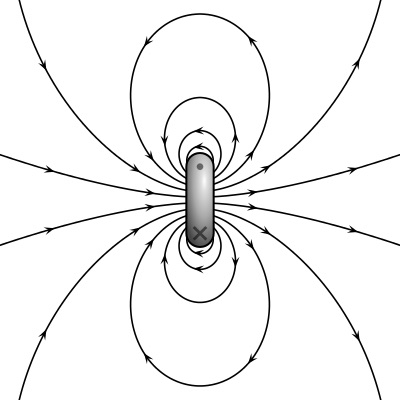
\includegraphics[width=\linewidth]{mag_dipole.jpg}
  \caption{Magnetic field around a loop of current}
  \label{fig:marginfig}
\end{marginfigure}
\section{Magnetic Force Between Two Parallel Wires}
Consider the force between two parallel wires.
$$\frac{F_1}{l}=\frac{\mu_0I_1I_2}{2\pi a}$$
This force is attractive if the the currents are in the same direction and repulsive if the wires are in opposite directions.

\section{Ampere's Law}
Ampere's law is the elegant representation describing the magnetic field around a current $I$.  We use an Amperian loop $s$ as a tool to determine the magnetic field 
$$\sum_{closed} \overrightarrow{B}\cdot \Delta\overrightarrow{s}=\mu_0I$$ 
The line integral of $\overrightarrow{B}\cdot \Delta\overrightarrow{s}$ around any closed path equals $\mu_0I$, where I is the total steady state current 
passing through any surface bounded by the closed path Amperian loop.
\subsection{Symmetric Path and Field}
If the field is uniform along the closed path then the summation reduces.
$$BS=\mu_0I$$ 
\section{B Field Inside a Solenoid}
A solenoid is a winding loop of current.  The magnetic field inside a solenoid maybe easily determined using Ampere's law using a rectangular loop of length $l$.
$$\sum_{closed} \overrightarrow{B}\cdot \Delta \overrightarrow{s}=Bl$$
$N$ is the number of winding turns through the loop.
$$Bl=\mu_0NI$$
It reduces to a linear dependence on the the density of turns per unit length $n$.
$$B=\mu_0nI$$

\section{Magnetic Flux}
Magnetic flux is defined as the total amount of magnetic field going through a surface.
$$\Phi_B=\sum \overrightarrow{B}\cdot d \overrightarrow{A}$$
The total magnetic flux going through a closed surface is zero.  This is known as Gauss's law for magnetism.
$$\sum_{closed} \overrightarrow{B}\cdot \Delta\overrightarrow{A}=0$$

\section{Displacement Current}
Displacement current is the effective current generated at a capacitor gap.  It is proportional to the time rate of change of electric flux.
$$I_d\equiv\epsilon_0\frac{d\Phi_E}{dt}$$
Since Ampere's law involves determining the current flux though the membrane bound by the Amperian loop is is possible to stretch the membrane so that it passed through the capacitor gap, where no actual current would pass through the membrane.  Therefore an increasing electric field must be considered equivalent to a real current.
$$\sum_{closed} \overrightarrow{B}\cdot \Delta \overrightarrow{s}=\mu_0(I+I_d)$$
An increasing electric field generates a magnetic field around it.  Therefore Ampere law requires a small addendum to include the displacement current.

